% The contents of this file is 
% Copyright (c) 2009-  Charles R. Severance, All Righs Reserved

\chapter{Programas en red}

A pesar de que muchos de los ejemplos de este libro se han dirigido a la lectura
de ficheros y a la búsqueda de datos dentro de ellos, existen otras muchas fuentes
distintas de información si también se tiene en cuenta Internet.

En este capítulo, fingiremos ser un navegador web y recuperaremos páginas
web usando el Protocolo de Transporte de Hipertexto ({\tt HyperText Transport Protocol} - HTTP).
Luego revisaremos los datos de esas páginas web y los analizaremos.

\section{Protocolo de Transporte de Hipertexto - HTTP}

El protocolo de red que hace funcionar la web es en realidad bastante simple, y
existe un soporte integrado en Python que se llama {\tt sockets} que hace que resulte muy
fácil realizar conexiones de red y recuperar datos a través de esas
conexiones desde un programa Python.

Un {\bf socket} es muy parecido a un archivo, excepto que un único socket
proporciona una conexión de doble sentido entre dos programas.
Es posible tanto leer como escribir en el mismo socket. Si se escribe algo en
un socket, es enviado hacia la aplicación que está al otro lado del socket. Si se lee
desde un socket, se obtienen los datos que la otra aplicación ha enviado.

Pero si intentas leer de un socket cuando el programa que está al otro lado
no ha enviado ningún dato---puedes esperar sentado. Si los programas de ambos extremos
del socket simplemente intentan recibir datos sin que ninguno envíe nada, esperarán durante mucho,
mucho tiempo.

De modo que una parte importante de la comunicación de programas a través de Internet consiste en tener algún
tipo de protocolo. Un protocolo es un conjunto de reglas precisas que determinan quién
empieza primero, qué debe hacer, cuáles son las respuestas siguientes para ese mensaje,
quién envía a continuación y todo lo demás. En cierto sentido las aplicaciones a ambos lados del
socket están interpretando un baile y cada una de ellas debe estar segura de que no pisa
los pies del otro.

Hay muchos documentos que describen esos protocolos de red. El Protocolo de Transporte de
Hipertexto está descrito en el siguiente documento:

\url{http://www.w3.org/Protocols/rfc2616/rfc2616.txt}

Se trata de un documento de 176 páginas, largo y complejo, con un montón de detalles. Si lo
encuentras interesante, no dudes en leerlo completo. Pero si echas un vistazo alrededor de la
página 36 del RFC2616, encontrarás la sintaxis para las peticiones GET. Para pedir un documento a un
servidor web, hacemos una conexión al servidor {\tt www.py4inf.com} en el puerto 80, y luego
enviamos una línea como esta

{\tt GET http://www.py4inf.com/code/romeo.txt HTTP/1.0 }

en la cual el segundo parámetro es la página web que estamos solicitando, y a continuación
enviamos una línea en blanco. El servidor web responderá con una cabecera que contiene cierta
información acerca del documento y una línea en blanco,
seguido por el contenido del documento.

\section{El Navegador Web Más Sencillo del Mundo}

Tal vez el modo más fácil de mostrar cómo funciona el protocolo HTTP sea escribir un
programa en Python muy sencillo, que realice una conexión con un servidor web y siga
las reglas de ese protocolo para solicitar\ un documento
y mostrar lo que el servidor le devuelve.

\beforeverb
\begin{verbatim}
import socket

misock = socket.socket(socket.AF_INET, socket.SOCK_STREAM)
misock.connect(('www.py4inf.com', 80))
misock.send('GET http://www.py4inf.com/code/romeo.txt HTTP/1.0\n\n')

while True:
    datos = misock.recv(512)
    if ( len(datos) < 1 ) :
        break
    print datos

misock.close()
\end{verbatim}
\afterverb
%
En primer lugar el programa realiza una conexión con el puerto 80 del
servidor \url{www.py4inf.com}.
Dado que nuestro programa está realizando el papel de ``servidor web'', el
protocolo HTTP dice que debemos enviar el comando GET seguido por una línea en blanco.

\beforefig
\centerline{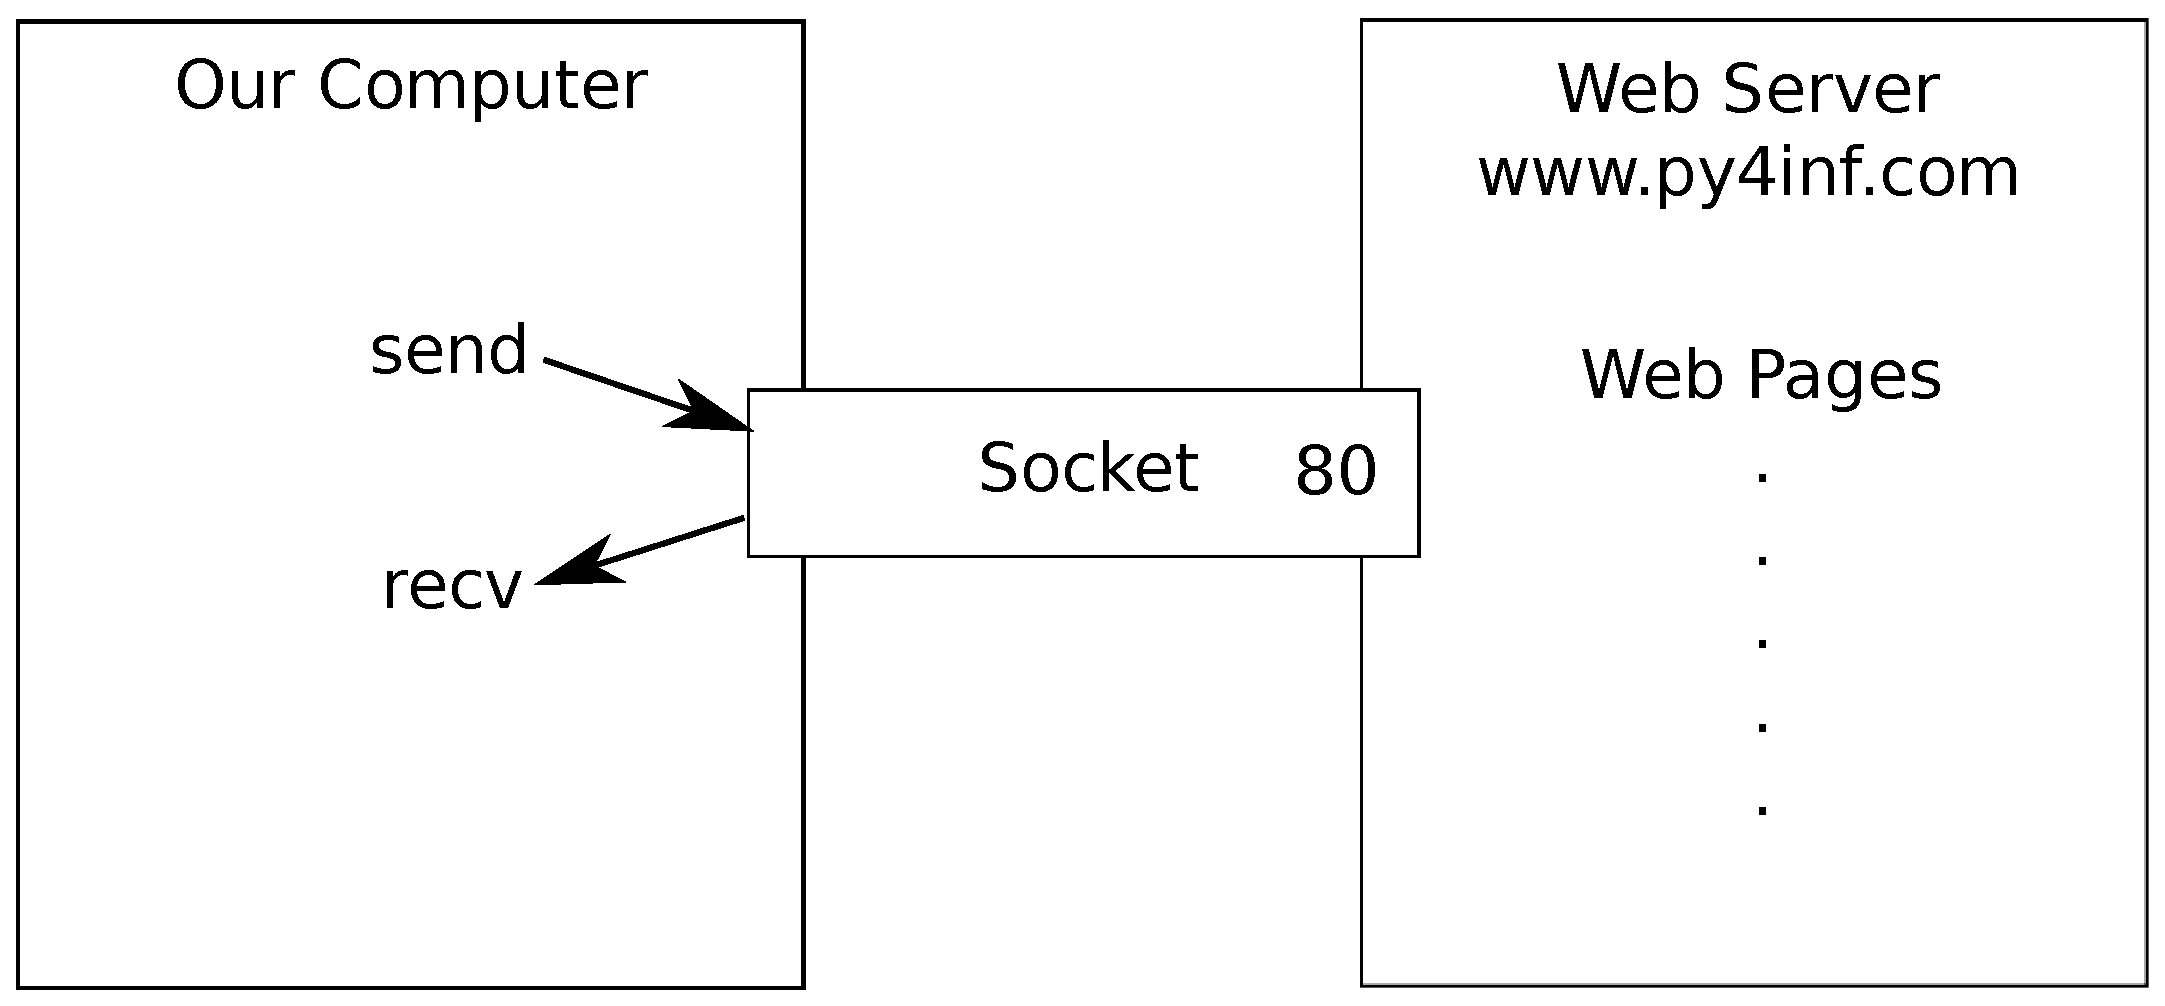
\includegraphics[height=1.50in]{figs2/socket.eps}}
\afterfig

Una vez enviada esa línea en blanco, escribimos un bucle que recibe los datos
desde el socket en bloques de 512 caracteres y los imprime en pantalla
hasta que no quedan más datos por leer (es decir, hasta que recv() devuelve
una cadena vacía).

El programa produce la salida siguiente:

\beforeverb
\begin{verbatim}
HTTP/1.1 200 OK
Date: Sun, 14 Mar 2010 23:52:41 GMT
Server: Apache
Last-Modified: Tue, 29 Dec 2009 01:31:22 GMT
ETag: "143c1b33-a7-4b395bea"
Accept-Ranges: bytes
Content-Length: 167
Connection: close
Content-Type: text/plain

But soft what light through yonder window breaks
It is the east and Juliet is the sun
Arise fair sun and kill the envious moon
Who is already sick and pale with grief
\end{verbatim}
\afterverb
%
La salida comienza con las cabecera que el servidor web envía
para describir el documento.
Por ejemplo, la cabecera {\tt Content-Type} indica que
el documento es del tipo texto sin formato ({\tt text/plain}).

Después de que el servidor nos envía la cabecera, añade una línea en blanco
para indicar el final de la misma, y a continuación envía los datos
reales del fichero {\tt romeo.txt}.

Este ejemplo nos muestra cómo crear una conexión de red de bajo nivel
con sockets. Los sockets pueden ser usados para comunicarse con un servidor
web, con un servidor de correo, o con muchos otros tipos de servidores.
Todo lo que se necesita es localizar el documento que describe
el protocolo correspondiente y escribir el código para enviar y recibir los datos
de acuerdo a ese protocolo.

Sin embargo, como el protocolo que se usa con más frecuencia es
el protocolo web HTTP, Python posee una librería
especial específicamente diseñada para trabajar con ese protocolo
y recibir documentos y datos a través de la web.

\section{Recepción de una imagen mediante HTTP}

\index{imagen!jpg}
\index{jpg}
En el ejemplo anterior, hemos recibido un archivo de texto sin formato,
que tenía saltos de línea en su interior, y lo único que hemos hecho
desde el programa ha sido ir copiando los datos en la pantalla. Podemos usar un programa
similar para recibir una imagen a través de HTTP. En lugar
de copiar los datos a la pantalla según va funcionando el programa,
acumularemos esos datos en una cadena, recortaremos las cabeceras,
y luego guardaremos los datos de la imagen en un archivo, como se muestra a continuación:

\beforeverb
\begin{verbatim}
import socket
import time

misock = socket.socket(socket.AF_INET, socket.SOCK_STREAM)
misock.connect(('www.py4inf.com', 80))
misock.send('GET http://www.py4inf.com/cover.jpg HTTP/1.0\n\n')


contador = 0
imagen = "";
while True:
    datos = misock.recv(5120)
    if ( len(datos) < 1 ) : break
    # time.sleep(0.25)
    contador = contador + len(datos)
    print len(datos),contador
    imagen = imagen + datos

misock.close()

# Búsqueda del final de la cabecera (2 CRLF)
pos = imagen.find("\r\n\r\n");
print 'Tamaño de cabecera',pos
print imagen[:pos]

# Saltar detrás de la cabecera y guardar los datos de la imagen
imagen = imagen[pos+4:]
manf = open("cosa.jpg","wb")
manf.write(imagen);
manf.close()
\end{verbatim}
\afterverb
%
Cuando el programa se ejecuta, produce la salida siguiente:

\beforeverb
\begin{verbatim}
$ python urljpeg.py 
2920 2920
1460 4380
1460 5840
1460 7300
...
1460 62780
1460 64240
2920 67160
1460 68620
1681 70301
Tamaño de cabecera 240
HTTP/1.1 200 OK
Date: Sat, 02 Nov 2013 02:15:07 GMT
Server: Apache
Last-Modified: Sat, 02 Nov 2013 02:01:26 GMT
ETag: "19c141-111a9-4ea280f8354b8"
Accept-Ranges: bytes
Content-Length: 70057
Connection: close
Content-Type: image/jpeg
\end{verbatim}
\afterverb
%
Puedes observar que, para esta url, la
cabecera {\tt Content-Type} indica que el
cuerpo del documento es una imagen ({\tt image/jpeg}).
Una vez que el programa termina, se pueden ver los datos de la imagen abriendo
el archivo {\tt cosa.jpg} con un visor de imágenes.

Al ejecutar el programa, se puede ver que no se obtienen 5120 caracteres
cada vez que que se llama al método {\tt recv()}.
Se obtienen tantos caracteres como hayan sido transferidos por el servidor web hacia nosotros
a través de la red en el momento de la llamada a {\tt recv()}.
En este ejemplo, se obtienen 1460 ó 2920 caracteres cada vez que
se solicita un máximo de 5120 caracteres de datos.

Los resultados obtenidos pueden ser diferentes dependiendo de la velocidad de tu red. Además
fíjate en que en la última llamada a {\tt recv()} se obtienen 1681 bytes, que es el final
de la cadena, y en la siguiente llamada a {\tt recv()} se obtiene una cadena de
longitud cero que nos indica que el servidor ya ha llamado a {\tt close()} en su lado
del socket, y por tanto no quedan más datos pendientes.

\index{time}
\index{time.sleep}
Podemos retardar las llamadas sucesivas a {\tt recv()} descomentando la llamada
a {\tt time.sleep()}. Así, esperamos un cuarto de segundo después de cada llamada,
de modo que el servidor puede ``adelantarse'' a nosotros y enviarnos más datos
antes de que llamemos de nuevo a {\tt recv()}. Con el retraso, esta vez el programa
se ejecuta así:
\beforeverb
\begin{verbatim}
$ python urljpeg.py 
1460 1460
5120 6580
5120 11700
...
5120 62900
5120 68020
2281 70301
Tamaño de cabecera 240
HTTP/1.1 200 OK
Date: Sat, 02 Nov 2013 02:22:04 GMT
Server: Apache
Last-Modified: Sat, 02 Nov 2013 02:01:26 GMT
ETag: "19c141-111a9-4ea280f8354b8"
Accept-Ranges: bytes
Content-Length: 70057
Connection: close
Content-Type: image/jpeg
\end{verbatim}
\afterverb
%
Ahora todas las llamadas a {\tt recv()}, excepto la primera y la última,
nos dan 5120 caracteres cada vez que solicitamos más datos.

Existe un buffer entre el servidor que hace las peticiones {\tt send()}
y nuestra aplicación que hace las peticiones {\tt recv()}. Cuando ejecutamos
el programa con el retraso activado, en algún momento el servidor podría
llenar el buffer del socket y verse forzado a detenerse hasta que
nuestro programa empiece a vaciar ese buffer. La detención de la aplicación
que envía los datos o de la que los recibe se llama
``control de flujo''.
\index{control de flujo}

\section{Recepción de páginas web con {\tt urllib}}

\index{urllib!imagen}
A pesar de que es posible enviar y recibir datos manualmente a través de HTTP
usando la librería socket, existe en Python un modo mucho más sencillo de
realizar esta habitual tarea,
mediante el uso de la librería {\tt urllib}.

Al usar {\tt urllib},
es posible tratar una página web de forma mucho más parecida a un fichero. Se puede
indicar simplemente qué página web se desea recuperar y
{\tt urllib} se encargará de gestionar todo lo referente al protocolo HTTP y
los detalles de la cabecera.

El código equivalente para leer el fichero {\tt romeo.txt}
desde la web usando {\tt urllib} es el siguiente:

\beforeverb
\begin{verbatim}
import urllib

manf = urllib.urlopen('http://www.py4inf.com/code/romeo.txt')
for linea in manf:
   print linea.strip()
\end{verbatim}
\afterverb
%
Una vez que la página web ha sido abierta con
{\tt urllib.urlopen}, se puede tratar como
un archivo y leer a través de ella usando un
bucle {\tt for}.

Cuando el programa se ejecuta, en su salida
sólo vemos el contenido del fichero. Las cabeceras
siguen enviándose, pero el código de {\tt urllib}
se queda con ellas y sólo nos devuelve
los datos.

\beforeverb
\begin{verbatim}
But soft what light through yonder window breaks
It is the east and Juliet is the sun
Arise fair sun and kill the envious moon
Who is already sick and pale with grief
\end{verbatim}
\afterverb
%

Como ejemplo, podemos escribir un
programa para recuperar los datos de
{\tt romeo.txt} y calcular la frecuencia
de cada palabra del fichero, como se muestra a continuación:

\beforeverb
\begin{verbatim}
import urllib

contadores = dict()
manf = urllib.urlopen('http://www.py4inf.com/code/romeo.txt')
for linea in manf:
    palabras = linea.split()
    for palabra in palabras:
        contadores[palabra] = contadores.get(palabra,0) + 1   
print contadores
\end{verbatim}
\afterverb
%
De nuevo vemos que una vez abierta la página web
se puede leer como si se tratase de un fichero local.

\section{Análisis de HTML y rascado de la web}
\index{web!scraping}
\index{web!rascado}
\index{HTML!análisis de}

Uno de los usos más habituales de las capacidades de {\tt urllib} en Python
es {\bf rascar} ({\tt scrape}) la web. El ``web scraping'', o rascado de la web,
consiste en escribir un programa
que finge ser un navegador web y recupera páginas, examinando
luego los datos de esas páginas para encontrar ciertos patrones.

Por ejemplo, un motor de búsqueda como Google buscará en el código
de una página web, extraerá los enlaces a otras páginas y recuperará
esas páginas, extrayendo los enlaces que haya en ellas y así sucesivamente. Usando esta técnica,
las  {\bf arañas} de Google se mueven por casi todas las páginas de
la web.

Google utiliza también la frecuencia con que las páginas que encuentra enlazan
hacia una página concreta para calcular la ``importancia'' de
esa página, y la posición en la que debe aparecer dentro de sus resultados de búsqueda.

\section{Análisis de HTML mediante expresiones regulares}

Un modo sencillo de analizar HTML consiste en utilizar expresiones regulares para
hacer búsquedas repetidas que extraigan subcadenas coincidentes con un modelo concreto.

Aquí tenemos una página web sencilla:

\beforeverb
\begin{verbatim}
<h1>La Primera Página</h1>
<p>
Si te apetece, puedes visitar la
<a href="http://www.dr-chuck.com/page2.htm">
Segunda Página</a>.
</p>
\end{verbatim}
\afterverb
%
Podemos construir una expresión regular bien formada que busque
y extraiga los valores de los enlaces del texto anterior, de éste modo:

\beforeverb
\begin{verbatim}
href="http://.+?"
\end{verbatim}
\afterverb
%
Nuestra expresión regular busca cadenas que comiencen por
``href="http://'', seguido de uno o más caracteres
(``.+?''), seguidos por otra comilla doble. El signo de interrogación
añadido a ``.+?'' indica que la coincidencia debe ser hecha
en modo ``no-codicioso'', en vez de en modo ``codicioso''.
Una búsqueda no-codiciosa intenta encontrar la cadena coincidente
{\em más pequeña} posible, mientras que una búsqueda codiciosa intentaría
localizar la cadena coincidente {\em más grande}.
\index{codicioso}
\index{no codicioso}

Añadimos paréntesis a nuestra expresión regular para indicar
qué parte de la cadena localizada queremos extraer, y
obtenemos el siguiente programa:
\index{regex!paréntesis}
\index{paréntesis!expresiones regulares}

\beforeverb
\begin{verbatim}
import urllib
import re

url = raw_input('Introduzca - ')
html = urllib.urlopen(url).read()
enlaces = re.findall('href="(http://.*?)"', html)
for enlace in enlaces:
    print enlace
\end{verbatim}
\afterverb
%
El método {\tt findall} de las expresiones regulares nos proporciona una lista de todas
las cadenas que coinciden con nuestra expresión regular, devolviendo sólo
el texto del enlace situado dentro de las comillas dobles.

Cuando ejecutamos el programa, obtenemos la siguiente salida:

\beforeverb
\begin{verbatim}
python urlregex.py 
Introduzca - http://www.dr-chuck.com/page1.htm
http://www.dr-chuck.com/page2.htm

python urlregex.py 
Introduzca - http://www.py4inf.com/book.htm
http://www.greenteapress.com/thinkpython/thinkpython.html
http://allendowney.com/
http://www.py4inf.com/code
http://www.lib.umich.edu/espresso-book-machine
http://www.py4inf.com/py4inf-slides.zip
\end{verbatim}
\afterverb
%
Las expresiones regulares funcionan muy bien cuando el HTML está bien formado
y es predecible. Pero dado que ahí fuera hay muchas páginas con HTML ``defectuoso'',
una solución usando solamente expresiones regulares puede, o bien
perder parte de los enlaces correctos, o bien terminar obteniendo datos erróneos.

Esto se puede resolver usando una librería de análisis de HTML robusta.

\section{Análisis de HTML mediante BeautifulSoup}
\index{BeautifulSoup}

Hay una cantidad considerable de librerías en Python que pueden ayudarte a analizar
HTML y a extraer datos de las páginas. Cada una de las librerías
tiene sus puntos fuertes y flacos, de modo que puedes elegir una
basada en tus necesidades.

Por ejemplo, vamos a analizar simplemente una entrada HTML cualquiera
y a extraer enlaces usando la librería {\bf BeautifulSoup}.
El código de BeautifulSoup se puede descargar e instalar
desde:

\url{http://www.crummy.com/software/}

Se puede descargar e ``instalar'' BeautifulSoup, o
simplemente colocar el archivo {\tt BeautifulSoup.py} en la
misma carpeta que nuestra aplicación.

A pesar de que el HTML se parece al XML\footnote{El formato XML será descrito
en el próximo capítulo.} y que algunas páginas están cuidadosamente
construidas para ser XML, la mayoría del HTML generalmente está
incompleto, de modo que provoca que un analizador de XML rechace la página completa de HTML
por estar formada inadecuadamente. BeautifulSoup tolera el HTML
aunque éste sea muy defectuoso, y aún en ese caso permite extraer los datos que se necesiten.

Vamos a usar {\tt urllib} para leer la página y luego usaremos
{\tt BeautifulSoup} para extraer los atributos {\tt href} de las
etiquetas de anclaje ({\tt a}).
\index{BeautifulSoup}
\index{HTML}
\index{análisis!HTML}

\beforeverb
\begin{verbatim}
import urllib
from BeautifulSoup import *

url = raw_input('Introduzca - ')
html = urllib.urlopen(url).read()
sopa = BeautifulSoup(html)

# Recupera todas las etiquetas de anclaje
etiquetas = sopa('a')
for etiqueta in etiquetas:
   print etiqueta.get('href', None)
\end{verbatim}
\afterverb
%
El programa solicita una dirección web, luego abre la página
web, lee los datos y se los pasa al analizador BeautifulSoup,
que recupera todas las etiquetas de anclaje e imprime en pantalla
el atributo {\tt href} de cada una de ellas.

Cuando el programa se ejecuta, muestra lo siguiente:

\beforeverb
\begin{verbatim}
python urllinks.py 
Introduzca - http://www.dr-chuck.com/page1.htm
http://www.dr-chuck.com/page2.htm

python urllinks.py 
Introduzca - http://www.py4inf.com/book.htm
http://www.greenteapress.com/thinkpython/thinkpython.html
http://allendowney.com/
http://www.si502.com/
http://www.lib.umich.edu/espresso-book-machine
http://www.py4inf.com/code
http://www.pythonlearn.com/
\end{verbatim}
\afterverb
%
Se puede utilizar BeautifulSoup para extraer varias partes de cada
etiqueta de este modo:

\beforeverb
\begin{verbatim}
import urllib
from BeautifulSoup import *

url = raw_input('Introduzca - ')
html = urllib.urlopen(url).read()
sopa = BeautifulSoup(html)

# Recupera todas las etiquetas de anclaje
etiquetas = sopa('a')
for etiqueta in etiquetas:
   # Busca las partes de una etiqueta
   print 'ETIQUETA:',etiqueta
   print 'URL:',etiqueta.get('href', None)
   print 'Contenido:',etiqueta.contents[0]
   print 'Atributos:',etiqueta.attrs
\end{verbatim}
\afterverb
%
Esto produce la siguiente salida:

\beforeverb
\begin{verbatim}
python urllink2.py 
Introduce - http://www.dr-chuck.com/page1.htm
ETIQUETA: <a href="http://www.dr-chuck.com/page2.htm">
Second Page</a>
URL: http://www.dr-chuck.com/page2.htm
Contenido: [u'\nSecond Page']
Atributos: [(u'href', u'http://www.dr-chuck.com/page2.htm')]
\end{verbatim}
\afterverb
%
Estos ejemplos tan sólo insinúan la potencia de BeautifulSoup
en el análisis del HTML. Lee la documentación y
los ejemplos que están en
\url{http://www.crummy.com/software/BeautifulSoup/} para obtener más detalles.

\section{Lectura de archivos binarios mediante urllib}

A veces se quiere recuperar un fichero que no es de texto (binario), como
un archivo de imagen o de video. Normalmente no resulta útil imprimir los datos de
estos ficheros, pero se puede hacer una copia de una URL en un archivo
local de nuestro disco duro con facilidad, usando {\tt urllib}.
\index{fichero!binario}

La pauta a seguir consiste en abrir la URL y usar {\tt read} para descargar el contenido
completo del documento en una variable de tipo cadena ({\tt img}), y luego escribir la
información a un archivo local, como se muestra a continuación:

\beforeverb
\begin{verbatim}
img = urllib.urlopen('http://www.py4inf.com/cover.jpg').read()
manf = open('portada.jpg', 'w')
manf.write(img)
manf.close()
\end{verbatim}
\afterverb
%
Este programa lee todos los datos de una sola vez a través de la red y los
almacena en la variable {\tt img} en la memoria principal de tu equipo,
luego abre el fichero {\tt portada.jpg} y escribe los datos en el
disco. Esto funcionará sólo si el tamaño del fichero es menor que el tamaño
de la memoria de tu PC.

Sin embargo, si se trata de un fichero enorme de audio o video, el programa puede fallar,
o al menos funcionar extremadamente lento cuando el equipo se quede sin memoria.
Para evitar agotar la memoria, vamos a recuperar los datos en bloques
(o buffers), y luego escribiremos cada bloque en el disco antes de recuperar
el siguiente. De este modo el programa podrá leer archivos de cualquier tamaño sin
usar toda la memoria del equipo.

\beforeverb
\begin{verbatim}
import urllib

img = urllib.urlopen('http://www.py4inf.com/cover.jpg')
manf = open('portada.jpg', 'w')
tamano = 0
while True:
    info = img.read(100000)
    if len(info) < 1 : break
    tamano = tamano + len(info)
    manf.write(info)

print tamano,'caracteres copiados.'
manf.close()
\end{verbatim}
\afterverb
%
En este ejemplo, leemos solamente 100.000 caracteres cada vez y luego
escribimos esos caracteres en el archivo {\tt portada.jpg},
antes de recuperar los 100.000 caracteres siguientes de datos desde
la web.

El programa funciona de este modo:

\beforeverb
\begin{verbatim}
python curl2.py 
568248 caracteres copiados.
\end{verbatim}
\afterverb
%

Si tienes un equipo con Unix o Macintosh, probablemente tendrás un comando
incorporado en tu sistema operativo que puede realizar esa misma operación
de este modo:
\index{curl}

\beforeverb
\begin{verbatim}
curl -O http://www.py4inf.com/cover.jpg
\end{verbatim}
\afterverb
%
El comando {\tt curl} es la abreviatura de ``copy URL'' y por eso estos dos
ejemplos se han llamado astutamente {\tt curl1.py} y {\tt curl2.py} en
\url{www.py4inf.com/code}, ya que implementan una funcionalidad similar
a la del comando {\tt curl}. Existe también un programa de ejemplo {\tt curl3.py}
que realiza la misma tarea de forma un poco más eficiente, en caso de
que quieras usar de verdad este diseño en algún programa que estés escribiendo.

\section{Glosario}

\begin{description}

\item[BeautifulSoup:] Una librería Python para analizar documentos HTML
y extraer datos de ellos,
que compensa la mayoría de las imperfecciones que los navegadores HTML
normalmente ignoran.
Puedes descargar el código de BeautifulSoup
desde
\url{www.crummy.com}.
\index{BeautifulSoup}

\item[puerto:] Un número que generalmente indica con qué aplicación
estás contactando cuando realizas una conexión con un socket en un servidor.
Por ejemplo, el tráfico web normalmente usa el puerto 80, mientras que el tráfico
del correo electrónico usa el puerto 25.
\index{puerto}

\item[rastrear:] La acción de un motor de búsqueda web que consiste en recuperar una página
y luego todas las páginas enlazadas por ella, continuando así sucesivamente hasta que
tienen casi todas las páginas de Internet, que
usan a continuación para construir su índice de búsqueda.
\index{spider}
\index{rastrear}

\item[socket:] Una conexión de red entre dos aplicaciones,
en la cual dichas aplicaciones pueden enviar y recibir datos en ambas direcciones.
\index{socket}

\item[scrape (rascado):] Cuando un programa simula ser un navegador web y
recupera una página web, para luego realizar una búsqueda en su contenido.
A menudo los programas siguen los enlaces en una página para encontrar la
siguiente, de modo que pueden atravesar una red de páginas o una red social.
\index{scrape}
\index{rascado}

\end{description}

\section{Ejercicios}

\begin{ex}
Cambia el programa del socket {\tt socket1.py} para que le pida al usuario
la URL, de modo que pueda leer cualquier página web.
Puedes usar {\tt split('/')} para dividir la URL en las partes que la componen,
de modo que puedas extraer el nombre del host para la llamada a {\tt connect} del socket.
Añade comprobación de errores, usando {\tt try} y {\tt except} para contemplar la posibilidad
de que el usuario introduzca una URL mal formada o inexistente.  
\end{ex}

\begin{ex}
Cambia el programa del socket para que cuente el número de caracteres que ha recibido
y se detenga, con un texto en pantalla, después de que se hayan mostrado 3000 caracteres. El programa
debe recuperar el documento completo y contar el número total de caracteres,
mostrando ese total al final del documento.
\end{ex}

\begin{ex}
Usa {\tt urllib} para rehacer el ejercicio anterior de modo que (1) reciba el documento
de una URL, (2) muestre hasta 3000 caracteres, y (3) cuente la cantidad total
de caracteres en el documento. No te preocupes de las cabeceras en este ejercicio,
muestra simplemente los primeros 3000 caracteres del contenido del documento.
\end{ex}

\begin{ex}
Cambia el programa {\tt urllinks.py} para extraer y contar
las etiquetas de párrafo (p) del documento HTML recuperado y
mostrar el total de párrafos como
salida del programa.
No muestres el texto de los párrafos, sólo cuéntalos.
Prueba el programa en varias páginas web pequeñas,
y también en otras más grandes.
\end{ex}

\begin{ex}
(Avanzado) Cambia el programa del socket, de modo que sólo muestre los datos
después de que se haya recibido la cabecera y la línea en blanco. Recuerda que {\tt recv}
va recibiendo caracteres (saltos de línea incluidos), y no líneas.
\end{ex}